\chapter{\tt gtk+ 移植}
\section{实验目的}
\begin{itemize}\itemsep=-3pt
  \item 学习GNU 开源软件的一般移植方法
\end{itemize}

\section{gtk+ 的背景}
    gtk+ 是一款跨平台的图形用户接口组件工具包, 原是 GIMP Toolkit 的缩写(GIMP 是
GNU Image Manipulation Program 的缩写, Linux中重要的图像处理软件, 类似Windows
中的photoshop), 以GPL版权协议发布, 是 Linux 系统中使用最为广泛的图形工具之一,
许多桌面系统都建立在 gtk+ 基础上, 如著名的 Gnome、xfce4.(另一款与之齐名的GUI
是Qt).

    gtk+ 不直接和显示硬件设备打交道.~Linux 桌面系统通常基于 X-Window.~而在
嵌入式应用中, 作为全功能 X 窗口系统的替代方案, 可以选择DirectFB作为后端. 

\begin{figure}
  \centering
  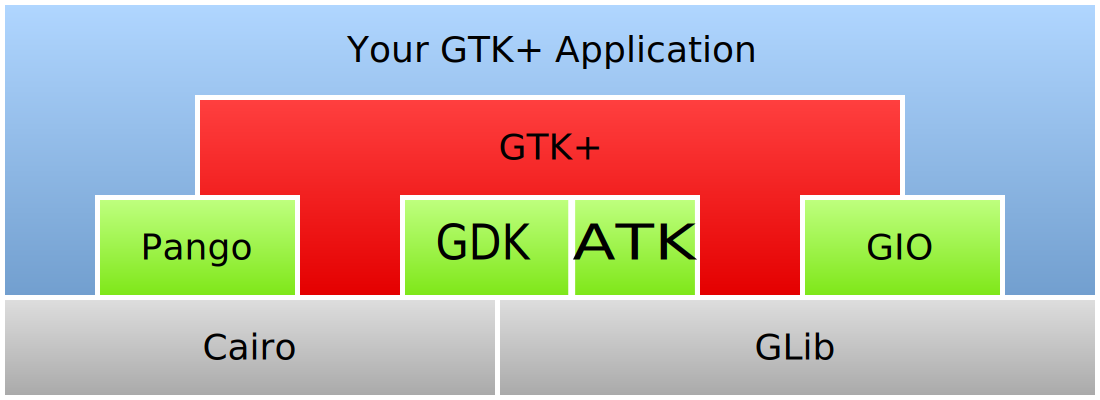
\includegraphics[width=.8\textwidth]{GTK+_architecture}
  \caption{基于gtk+的软件层次结构}\label{fig_gtk}
\end{figure}

\section{gtk 库的依赖关系}
从图\ref{fig_gtk}\footnote{图片引自 en.wikipedia.org/wiki}中可以看到, 
gtk+ 除了为上层应用提供接口函数库以外, 自身也依赖一系列的更底层的库.~
图\ref{fig_gtkdfb}是建立gtk+的库依赖关系.~我们需要根据
这样的依赖关系逐层构造系统的API.

\begin{figure}
  \centering
  \includegraphics[width=.8\textwidth]{gtk_dependency}
  \caption{gtk+的软件依赖关系}\label{fig_gtkdfb}
\end{figure}

    本实验中, 我们的最终目标是编译出 gtk+-2.16.6 的库以及演示程序gtk-demo.
~以下根据依赖关系, 对各个库加以简单的说明.~版本号是本实验建议版本.
\begin{itemize}
  \item zlib-1.2.8. zlib 是 Linux 系统最基本的压缩/解压库, 许多软件都会直接
      或间接地用到它.~zlib 仅依赖 glibc.~针对 Linux系统的交叉编译工具链中已经
      包含了 glibc 的动态和静态库, 编译 zlib 时会自动链接.(Linux 系统中几乎
      所有软件都会链接 glibc, 下面不再特别说明)

  \item tslib-1.0.0. 触摸屏支持库, 提供人机交互接口的输入支持.~有关触摸屏库的
      说明和编译请参考触摸屏移植部分.

  \item libpng-1.2.24. PNG(Portable Network Graphics)是广泛应用于互联网的一种
      图像格式. libpng 依赖 zlib 库的压缩/解压功能.

  \item libjpeg-turbo-1.2.1. JPEG(Joint Photographic Experts Group), 非常
      著名的图像压缩标准格式.libjpeg 不依赖其它库.

  \item pixman-0.16.0. 底层像素处理工具(Pixel Manipulation).~可依赖于 gtk+,
      本实验在编译时禁止该依赖关系.

  \item libxml2-2.6.30/expat-2.0.1. XML(Extensible Markup Language, 扩展标记
      语言) 是在互联网中广泛使用的一种标记语言, 既可以让人读懂, 也能让机器
      读懂.~Linux 系统中的很多软件基于 xml 语言.~目前在Linux系统中, 提供 xml
      解释功能的主要有两套库:expat 和 libxml2.~多数软件依赖于 libxml2, 但
      仍有少数仅依赖 expat.~expat 不依赖其它软件, libxml2 可以依赖 zlib.

  \item dbus-1.8-16. D-Bus(Desktop BUS) 提供桌面环境下的进程间通信机制, 属于
      freedesktop.org 项目的一部分.~dbus 依赖 xml 库, 可选择 libxml 或者
      expat.~但由于 libxml 早已停止开发, 所以在编译dbus时指定连接 expat库.

  \item glib-2.26.1. glib 原始于gtk+计划.~在gtk+-2版本之前, 不属于图形用户
      接口部分的功能被从 gtk+ 中分离出来单独开发, 这部分就是glib.~glib 依赖
      dbus 和 zlib.

  \item freetype-2.3.7. freetype 库实现矢量字体TrueType、Type1显示效果支持
      (字体渲染). 在连接 libpng 时还可以支持 png 压缩的点阵字体.~freetype
      自身已包含 zlib 解压功能, 可以不依赖 zlib.~也可在编译时指定使用系统的
      zlib.

  \item fontconfig-2.6.0. 字体配置工具, 告诉系统如何找到字体库, 依赖freetype,
      可选择性地依赖 expat 或者 libxml2.

  \item DirectFB-1.4.1. Direct Frame Buffer 提供图形加速、输入抽象层处理以及
      窗口系统的基本功能, 是gtk+ 的后端.~它依赖触摸屏库tslib、字体库freetype
      以及图形库libpng、libjpeg.

  \item cairo-1.6.4. 基于2维矢量图形的工具包.~在本实验中, 除后端选择DirectFB外,
      还依赖 fontconfig、libxml2 和 pixman.
  \item atk-1.29.4. ATK (Accessibility Toolkit) 提供客户/服务器访问API实现.
      ~依赖 glib.

  \item pango-1.20.5. pango 用于将多语种的文字高质量地渲染输出, 后端依赖cairo
      和glib.
\end{itemize}

\section{编译过程}
\subsection{编译准备}
    主机准备好必要的编译工具, 包括针对目标系统的交叉编译工具链和主机的开发
工具(gcc、GNUmake、autoconf、libtool等).

    准备三个有权限的目录, 一个用于存放源码包, 一个用于编译, 一个用于存放编译
后生成的文件, 也就是目标系统运行所需的程序以及库.~下面的编译过程中, 基于如下
的目录结构

\begin{verbatim}
    /home/student/src/
    /home/student/build/
    /home/student/target/
\end{verbatim}

    源码包通常具有 .tar.gz、.tag.bz2、.tar.xz等后缀形式.~无论哪种压缩形式,
统一可以用 ``tar xf foo.tar.*''解压.

\subsection{一般方法}
\begin{enumerate}
  \item 解压\\
      进入 /home/student/build, 执行 tar xf ../src/foo.tar.bz2 将压缩包
      foo.tar.bz2 解压到当前目录.
  \item 获得 configure\\
      进入解压目录.
      大多数源码包解压后, 根目录上都会有一个 configure 文件, 该文件具备可执行
      属性. 如果这个文件不存在, 则应有一个 autogen.sh 文件, 或者有
      configure.ac 文件.~对于前者, 可以在该目录下执行``sh autogen.sh'',
      对于后者, 可以执行 ``autoreconf --ivf'', 均可生成 configure 文件.
  \item 获得 Makefile\\
      确定有 configure 文件后, 在该目录下执行``./configure'', 经过一系列的
      系统检查和配置工作, 便可生成Makefile.~Makefile 可能在各级子目录中都会
      存在, 我们只需要在根目录上看到有 Makefile 即表示配置成功.\\
      为了获得不同的编译结果 configure 命令包含了很多选项, 需要在执行命令的
      同时给出.~例如, 我们通常会这样执行配置命令:

    \begin{boxedminipage}{.8\textwidth}
        \begin{tabular}{ll}
            ./configure           &$\backslash$\\
            \qquad -{}-host=arm-linux      &$\backslash$\\
            \qquad -{}-prefix=/usr         &$\backslash$\\
            \qquad -{}-bindir=/usr/bin     &$\backslash$\\
            \qquad -{}-sbindir=/usr/sbin   &$\backslash$\\
            \qquad -{}-sysconfdir=/etc     &$\backslash$\\
            \qquad -{}-libexecdir=/usr/lib &$\backslash$\\
            \qquad -{}-localstatedir=/var  &$\backslash$\\
            \qquad -{}-disable-static      &$\backslash$\\
            \qquad -{}-enable-shared       &
        \end{tabular}
    \end{boxedminipage}

    该配置命令设置了软件运行环境, 指定交叉编译器前缀为``arm-linux-'', 编译共享
库, 不编译静态库.

  \item 编译和安装\\
      多数软件简单执行``make'' 便可完成编译工作, 部分软件需要在``make''命令
      后加上编译的目标项目.\\
      通常用 ``make install'' 完成软件安装.~在我们的实验中用 ``make install 
      DESTDIR=/home/student/target'' 安装, 将软件安装到DESTDIR 指定的
      安装目录, 否则, 按缺省方式会安装到 /usr 目录(``configure 选项
      -{}-prefix''), 而这个目录是主机系统的目录.

\end{enumerate}

\subsection{环境变量}
    由于库的依赖问题, 编译过程中需要知道已经存在的库在什么地方.~通过设置
环境变量 ``PKG\_CONFIG\_PATH'', 在configure时就可以很方便地找到它们:

    export PKG\_CONFIG\_PATH=/home/student/target/usr/lib/pkgconfig

    gcc 编译时需要知道已经安装的库的头文件在哪里, 可以通过``-I''指定目录,
将该路径交给环境变量``CFLAGS''.

    export CFLAGS="-I/home/student/target/usr/include"

    该变量中可以包含多个路径.如果是用g++编译, 该功能对应的变量名称是CPPFLAGS
或CXXFLAGS.

    gcc 链接时要为它指明库文件所在路径: 

    export LDFLAGS="-L/home/student/target/usr/lib"

    如果需要特别指明链接库, 用 LIBS 变量 ("-lfoo").
\subsection{一些特殊的设置}
    多数软件包都可以按照上面给出的``configure''形式配置和编译.~下面几个软件包
在配置或者编译时略有不同:
\begin{enumerate}
  \item zlib, 按下面的步骤编译\\
      CC=arm-linux-gcc\\
      ./configure -{}-shared -{}-prefix=/usr

  \item pixman, configure 增加一个选项 -{}-disable-gtk

  \item libxml2, configure 增加一个选项 -{}-without-python

  \item dbus,  configure 时另外再加上两个选项:\\
      -{}-without-dbus-glib  -{}-disable-tests

  \item glib, configure 增加以下四个选项:\\
          glib\_cv\_uscore=no\\
          glib\_cv\_stack\_grows=no\\
          ac\_cv\_func\_posix\_getpwuid\_r=yes \\
          ac\_cv\_func\_posix\_getgrgid\_r=yes\\
    说明:编译glib 需要检查目标运行环境的功能是否完备.~通常检查的方法是编写
    一段小程序, 测试看一下是否能编译通过, 或者测试编译后能否运行.~但交叉编译的
    结果在主机上是不能运行的.~如果在 configure 时提供预期的运行结果, 就可以
    避开编译测试过程.

  \item fontconfig, configure 时增加以下选项:\\
      -{}-with-arch=arm \\
      -{}-enable-libxml2 \\
      -{}-with-freetype-config=/home/student/target/usr/bin/freetype-config \\
      -{}-with-cache-dir=/var/cache/fontconfig \\
      -{}-with-default-fonts=/usr/share/fonts

  \item DirectFB, configure 时增加以下选项:\\
      -{}-disable-x11 \\
      -{}-disable-osx \\
      -{}-enable-zlib \\
      -{}-enable-jpeg \\
      -{}-with-gfxdrivers=none \\
      -{}-with-inputdrivers=keyboard,linuxinput,tslib \\
      TSLIB\_CFLAGS="-I/home/student/target/usr/include" \\
      TSLIB\_LIBS="-lts" \\
      FREETYPE\_CFLAGS="-I/home/student/target/usr/include/freetype2" \\
      FREETYPE\_LIBS="-lfreetype"

  \item cairo,  configure 时增加以下选项:\\
      -{}-disable-win32 \\
      -{}-disable-xlib \\
      -{}-enable-directfb \\
      -{}-enable-freetype \\
      FREETYPE\_CFLAGS="-I/home/student/target/usr/include/freetype2" \\
      FONTCONFIG\_CFLAGS="-I/home/student/target/usr/include/fontconfig" \\
      FONTCONFIG\_LIBS="-lfontconfig -lfreetype -lxml2 -lz"

  \item gtk+, 首先需要去除 gtk+ configure 中检查 pango 过程的代码.
      ~用编辑器打开 configure, 将30893到30899行删除.

     其次, 需要将 demos/gtk-demo/geninclude.pl.in 中 所有``defined''单词
     删除,避免高版本 perl 在处理该文件时产生语法错误.

     打完上面两个补丁, 再行编译, 仍然需要增加几个选项:\\
      -{}-with-gdktarget=directfb \\
      -{}-without-libjasper \\
      -{}-without-libtiff \\
      gio\_can\_sniff=yes

      如果之前编译了libjasper(JPEG2000库)和tiff(Tagged Image File Format),则
      上面两个``without''可以换成``with''.
\end{enumerate}

\subsection{编译技巧}
    软件移植的工作相当繁琐, 很多操作需要重复多次.~为避免重复劳动, 减少错误,
我们可以把一些程序化的工作写成脚本程序.~例如, 下面的脚本可以胜任多数软件编译:

\begin{boxedminipage}{.8\textwidth}
\setlength{\parindent}{0em}
   \#!/bin/bash\\ \ 

   export SOURCEPATH=/home/student/src

   export BUILDPATH=/home/student/build

   export INSTALLPATH=/home/student/target

   export PREFIX="-{}-host=arm-linux $\backslash$\\
      -{}-prefix=/usr    $\backslash$\\
      -{}-exec-prefix=/usr    $\backslash$\\
      -{}-sysconfdir=/etc   $\backslash$\\
      -{}-localstatedir=/var $\backslash$\\
      -{}-disable-static  $\backslash$\\
      -{}-enable-shared"

   export CFLAGS="-I\${INSTALLPATH}/usr/include"

   export CPPFLAGS="-I\${INSTALLPATH}/usr/include"

   export LDFLAGS="-L\${INSTALLPATH}/usr/lib"

   export PKG\_CONFIG\_PATH=\${INSTALLPATH}/lib/pkgconfig

   cd \$BUILDPATH

   tar xf ../src/\$1.tar.*

   cd \$1

   ./configure \${PREFIX} \$2

   make
   
   make install DESTDIR=\${INSTALLPATH}
\end{boxedminipage}

将其命名为 build.sh, 每次只要执行``sh build.sh pixman-0.16.0 -{}-disable-gtk''
就可以完成 pixman 的编译.~对那些编译格式特殊的软件, 或借助中间文件, 或利用脚本
传递参数, 或专门单独写一个脚本, 都可以大大提高开发效率.

\section{测试}
    gtk+ 编译完成后, 将 target/ 目录平移到目标系统, 保持子目录结构不变.~
此时 gtk-demo 应该在 /usr/bin 目录下.~由于字体和图形环境没有正确设置, 初次
运行会有一些不成功的提示信息.~请根据这些提示完善系统设置.

\section{实验要求}

\clearpage
